\documentclass{article}
\usepackage{graphicx} % Required for inserting images
\usepackage{ctex}
\usepackage{listings}
\usepackage{xcolor}
\usepackage{float}
\usepackage{hyperref}
\usepackage{booktabs} 
\usepackage{siunitx}
\usepackage{caption}
\usepackage{svg}

% 定义 R 语言的配色方案 (模仿 RStudio 风格)
\definecolor{r-bg}{RGB}{248,248,248}
\definecolor{r-frame}{RGB}{200,200,200}
\definecolor{r-keyword}{RGB}{180,0,150} % 函数名/关键词
\definecolor{r-string}{RGB}{150,0,0}    % 字符串
\definecolor{r-comment}{RGB}{0,128,0}   % 注释

\lstset{
    language=R,
    basicstyle=\ttfamily\footnotesize,  % 改成更小的字体
    keywordstyle=\color{r-keyword}\bfseries,
    commentstyle=\color{r-comment}\itshape,
    stringstyle=\color{r-string},
    showstringspaces=false,
    breaklines=true,
    numbers=left,
    numberstyle=\tiny\color{gray},
    frame=none,
    backgroundcolor=\color{r-bg}
}

% --- 链接美化 ---
\hypersetup{
    colorlinks=true,
    linkcolor=blue,
    filecolor=magenta,      
    urlcolor=cyan,
}

\title{实验一  差异表达分析}
\author{Yuchen Gao}
\date{March 2026}

\begin{document}

\maketitle

\section{实验目的}

\begin{enumerate}
    \item 了解RNA-seq的基本原理以及流程
    \item 了解基因差异表达分析的基本原理以及方法
    \item 了解假设检验原理与方法
    \item 了解多重假设检验校正原理与方法
    \item 掌握DESeq2工作流并实践
\end{enumerate}

\section{背景介绍}

\subsection{RNA-seq}

RNA测序技术（RNA-seq）通过二代测序（NGS）技术检查样本中RNA的数量和序列，。此技术能够分析转录组，揭示在特定条件下（如肿瘤 vs 正常组织）基因的开启、关闭状态及其表达水平。通过对比不同条件下的样本，研究者可以识别出由于生物学处理或疾病状态引起的基因表达变化。

\subsection{DEG}

基因差异表达（Differential gene expression,DEG）旨在将获得的RNA-seq结果进行分析，将多个实验组进行比较，以找出在不同条件下哪些基因/转录本发生了显著变化，例如癌细胞与正常细胞、药物处理组与对照组等等。

在DEG分析中，Fold Change（FC）是一个核心指标，用于衡量某个基因在两个不同条件之间表达量的变化大小，其计算方法为：$FC = \frac{B}{A}$（其中B为实验组某基因平均表达量，A为对照组该基因平均表达量）。通常表示为 $\log_2$ FC，以令数据更具有对称性，分布更接近正态分布，便于可视化。

进一步地，p值用于衡量所得到的不同基因的表达量是否具有显著性差异。$p < 0.05$被认为差异由随机误差导致的概率很低，因此两组中的基因显著差异表达。然而在处理较大的基因数量时，为防止出现的假阳性情况，将对结果进行多重检验校正，从而获得$padj$,控制假阳性所占比例

\subsection{TCGA}

癌症基因组图谱（TCGA）是由美国国家癌症研究所（NCI）和国家人类基因组研究所（NHGRI）于2006年联合启动的一项宏大计划，对33种不同类型的癌症进行系统的基因组表征。在这套数据中，不仅包含RNA-Seq（转录组），还包括 DNA 测序（突变）、甲基化、蛋白质组学（RPPA）和临床数据（生存期、病理分期）。TCGA研究网络已对大量人类肿瘤进行了特征分析，旨在揭示DNA、RNA、蛋白质及表观遗传层面的分子异常。

在本实验中，我们准备利用TCGA数据组中的RNA-seq的数据组，进行DEG分析的练习

\section{实验方法}

\subsection{选择肝细胞癌数据集进行DEG分析练习}

由上所述，考虑到数据集对照组严格、标准数据层级以及样本量庞大的特点，使用TCGA中的LIHC（Liver Hepatocellular Carcinoma，肝细胞癌） 数据集进行DEG分析练习。

本数据集在 TCGA 的所有癌种中，RNA-Seq数据质量相对稳定，测序深度较深，且受到的样本降解干扰相对较小。更重要的是，LIHC是GEPIA3等在线工具支持最完善的癌种之一，这意味着在R语言里算出的结果，可以立即在GEPIA3网页端进行二次验证。

\subsection{使用Bioconductor、tidyverse软件包}

Bioconductor是全球生物信息学领域的开源软件工程，用于转录组（RNA-seq）、单细胞或基因组分析，在本次分析练习中，利用了Bioconductor中org.Hs.eg.db、DESeq2、EnhancedVolcano的软件包。

\begin{itemize}
    \item DESeq2(1.50.2)：基因差异表达分析的核心算法
    \item org.Hs.eg.db(3.22.0)：人类基因注释数据库，用来翻译基因 ID，进行更好的可视化处理
    \item EnhancedVolcano(1.28.2)：用于绘制火山图
\end{itemize}

tidyverse(2.0.0)软件包用于整理基因的表达数据，为进行基因差异表达分析提供所需的表格

\subsection{命令、参数的意义}

\subsubsection{安装软件包}

\begin{lstlisting}[language=R]
if (!require("BiocManager")) install.packages("BiocManager")
BiocManager::install("The_software_packages_you_need")
\end{lstlisting}

\begin{lstlisting}[language=R]
install.packages()
\end{lstlisting}

\subsubsection{数据读取与预处理}

\begin{lstlisting}[language=R]

raw <- read.csv() # 读取文件
matrix_1 <- as.matrix() # 转换为matrix并命名
rownames(matrix_1) <- raw[]
cts <- round()  #数据转换
\end{lstlisting}

\subsubsection{制作DEG分析所需表格}

\begin{lstlisting}[language=R]
tcga_id <- colnames() # 获得基因名称
code <- substr() #获得状态信息
condition <- ifelse()
condition <- factor() # 将condition转换为factor
colData <- data.frame() # 制作样本类型数据框
\end{lstlisting}

\subsubsection{数据预处理与差异分析}

\begin{lstlisting}[language=R]
dds <- DESeqDataSetFromMatrix(countData = , colData = , design = ) # 构建差异分析数据集对象，design指定比较的实验因素
keep <- rowSums(counts(dds) )>= # 筛选总count>=10的基因
dds <- dds[keep,] # 使得dds里只包括有效表达的基因
dds <- DESeq(dds) # 执行差异表达分析
res <- results(dds, contrast=) # 提取对比结果
\end{lstlisting}

\subsubsection{结果整理}

\begin{lstlisting}[language=R]
resOrdered <- res[order(),] # 对结果 res 进行排列
summary()
\end{lstlisting}

\subsubsection{结果可视化}

基因ID转换

\begin{lstlisting}[language=R]
res_df <- as.data.frame() %>% rownames_to_column() # 将 DESeq2 的结果转为数据框，将行名变为列名
res_df$ENSEMBL_clean <- gsub() # 去掉 Ensembl ID 中的版本号，方便后续匹配数据库
gene_map <- bitr() # 转化为基因名称

\end{lstlisting}

绘图参数定义

\begin{lstlisting}[language=R]
# 定义筛选阈值
cut_off_pvalue = 
cut_off_logFC = 
# 提取最显著的15个基因方便后期标注
select_genes <- res_final %>%
  filter() %>%
  arrange() %>%
  head() %>%
  pull()
\end{lstlisting}

绘制火山图

\begin{lstlisting}[language=R]
EnhancedVolcano()
\end{lstlisting}

\section{实验结果}

\subsection{完整代码}

\begin{lstlisting}[language=R]
# --- 1. 环境准备 ---
if (!require("BiocManager", quietly = TRUE))
  install.packages("BiocManager")
BiocManager::install(version = "3.22")
BiocManager::install(c("GenomicFeatures", "AnnotationDbi"))
BiocManager::install("DESeq2")
BiocManager::install("org.Hs.eg.db")
BiocManager::install("EnhancedVolcano")


library(DESeq2)
library(tidyverse)
library(org.Hs.eg.db)
library(EnhancedVolcano)
library(ggplot2)
library(ggrepel)

packageVersion("DESeq2")
packageVersion("tidyverse")
packageVersion("org.Hs.eg.db")
packageVersion("EnhancedVolcano")

# --- 2. 数据读取与预处理 ---
raw <- read.csv("/Users/gaoyuchen/Downloads/TCGA-LIHC.star_counts (1).tsv", sep = "\t")
matrix_1 <- as.matrix(raw[, -1])
rownames(matrix_1) <- raw[, 1]
cts <- round(2^matrix_1 - 1) 

# --- 3. 构建分组信息 ---
tcga_id <- colnames(cts)
code <- substr(tcga_id, 14, 14)
condition <- ifelse(as.numeric(code) < 1, "tumor", "normal")
condition <- factor(condition, levels = c("normal", "tumor")) 

colData <- data.frame(row.names = tcga_id,tcga_id=tcga_id,code = code,condition = condition)

# --- 4. 差异分析 ---
dds <- DESeqDataSetFromMatrix(countData = cts, colData = colData, design = ~ condition)
keep <- rowSums(counts(dds))>= 10
dds <- dds[keep,]
dds <- DESeq(dds)
res <- results(dds, contrast=c("condition", "tumor", "normal"))
res

# ---5. 整理结果 ----
resOrdered <- res[order(res$pvalue),]
summary(res)
resOrdered

# --- 6. ID 转换与去重 ---
res_df <- as.data.frame(res) %>% 
  rownames_to_column("ENSEMBL_full") %>%
  mutate(ENSEMBL_clean = gsub("\\..*", "", ENSEMBL_full))

gene_map <- bitr(res_df$ENSEMBL_clean, 
                 fromType = "ENSEMBL", 
                 toType = "SYMBOL", 
                 OrgDb = org.Hs.eg.db, 
                 drop = FALSE)

res_final <- res_df %>%
  inner_join(gene_map, by = c("ENSEMBL_clean" = "ENSEMBL")) %>%
  filter(!is.na(SYMBOL)) 

res_final

# --- 7. 绘图参数定义 ---
cut_off_pvalue = 1e-5
cut_off_logFC = 2

select_genes <- res_final %>%
  filter(!is.na(padj)) %>%
  filter(padj < cut_off_pvalue & abs(log2FoldChange) > cut_off_logFC) %>%
  arrange(padj) %>%
  mutate(direction = ifelse(log2FoldChange > 0, "up", "down")) %>%
  group_by(direction) %>%
  slice_head(n = 5) %>%
  ungroup() %>%
  pull(SYMBOL)

# --- 7. 最终绘图 ---
EnhancedVolcano(res_final,
                lab = res_final$SYMBOL,
                x = "log2FoldChange",
                y = "padj",
                selectLab = select_genes,       
                pCutoff = cut_off_pvalue,
                FCcutoff = cut_off_logFC,
                arrowheads = FALSE,
                drawConnectors = TRUE,          
                widthConnectors = 0.8,          
                colConnectors = 'grey10',       
                lengthConnectors = unit(10, 'mm'), 
                max.overlaps = 20,             
                pointSize = 1.0,
                labSize = 3.5,                  
                labCol = 'black',
                labFace = 'bold',
                xlab = bquote(~Log[2]~ "Fold Change"),
                ylab = bquote(~-Log[10]~italic(P)),
                xlim = c(-10, 10),             
                ylim = c(0, max(-log10(res_final$padj), na.rm = TRUE) + 5),                
                legendLabels = c("NS", "Log2 FC", "P-value", "P-value & Log2 FC"),
                legendPosition = "top",
                legendLabSize = 10,
                title = "Volcano Plot: Tumor vs Normal",
                subtitle = paste0("Total genes: ", nrow(res_final)),
)

library(dplyr)
res_classified <- res_final %>%
  mutate(group = case_when(
    padj < cut_off_pvalue & log2FoldChange > cut_off_logFC ~ "Up",       
    padj < cut_off_pvalue & log2FoldChange < -cut_off_logFC ~ "Down",    
    padj < cut_off_pvalue & abs(log2FoldChange) <= cut_off_logFC ~ "P_only", 
    padj >= cut_off_pvalue & abs(log2FoldChange) > cut_off_logFC ~ "FC_only", 
    TRUE ~ "NS" 
  ))

gene_counts <- table(res_classified$group)
print(gene_counts)


# 提取上调基因的所有参数，并按显著性(padj)排序
up_table <- res_classified %>%
  filter(group == "Up") %>%
  select(SYMBOL, log2FoldChange, pvalue, padj) %>%
  arrange(padj)

# 提取下调基因的所有参数，并按显著性(padj)排序
down_table <- res_classified %>%
  filter(group == "Down") %>%
  select(SYMBOL, log2FoldChange, pvalue, padj) %>%
  arrange(padj)

print(head(up_table, 10))
print(head(down_table, 10))

write.csv(head(up_table, 10), 
          file = "/Users/gaoyuchen/Downloads/Top50_Up_Genes.csv", 
          row.names = FALSE)
write.csv(head(down_table, 10), 
          file = "/Users/gaoyuchen/Downloads/Top50_Down_Genes.csv", 
          row.names = FALSE)


\end{lstlisting}

\subsection{安装所需包并载入}

在代码1-20行完成了对于Bioconductor中DESseq2、org.Hs.eg.db以及EnhancedVolcano的安装，完成了tidyverse包的安装，并且成功展示其版本号

\begin{figure}[H]  % 注意这里是大写的 H
    \centering
    
\includegraphics[width=0.5\linewidth]{1.png}
    \caption{运行截图1}
    \label{fig:运行截图1}
\end{figure}

经过查验发现，所有软件包均处于当前Bioconductor稳定发行版的最新状态

\subsection{导入数据以及数据转换}

从\href{https://xenabrowser.net}{TCGA 网站}下载表达量数据并解压缩，然后通过代码21-26行，完成了数据的导入，数据框命名为raw。注意到官网给出，数据经过了$log2(count+1)$的处理，因此再通过实验方法中的命令行将数据转换为真正的基因表达量。

\begin{figure}[H]  % 注意这里是大写的 H
    \centering
    
\includegraphics[width=0.5\linewidth]{2.png}
    \caption{运行截图2}
    \label{fig:运行截图2}
\end{figure}

\begin{figure}[H]  % 注意这里是大写的 H
    \centering
    
\includegraphics[width=0.5\linewidth]{3.png}
    \caption{结果截图}
    \label{fig:结果截图}
\end{figure}

\begin{figure}[H]  % 注意这里是大写的 H
    \centering
    
\includegraphics[width=0.5\linewidth]{4.png}
    \caption{结果截图}
    \label{fig:结果截图}
\end{figure}

\subsection{生成样本类型数据框}

想要进行DEG分析，需要在有cts表格后，附加一个记录不同样本所对应状态的样本类数据框，在代码27-32行，完成了样本类数据框的生成。在这段代码中，成功提取了基因ID，并根据 TCGA 命名规范提取ID的第14位字符并利用其定义样本类型。进一步地，将字符向量转换为因子，并显式设置参考水平，以便于后续直接以Normal状态为对照组进行分析。

\begin{figure}[H]  % 注意这里是大写的 H
    \centering
    
\includegraphics[width=0.5\linewidth]{5.png}
    \caption{cts}
    \label{fig:cts}
\end{figure}

\begin{figure}[H]  % 注意这里是大写的 H
    \centering
    
\includegraphics[width=0.5\linewidth]{6.png}
    \caption{colData}
    \label{fig:colData}
\end{figure}

\subsection{构建 DESeqDataSet，预过滤以及差异分析}

此过程由代码第35-41行完成。构建DESeqDataSet，旨在将基因表达矩阵、样本类型数据框以及实验设计打包，是后续进行DEG处理的必经之路。

之后，成功筛选总count>=10的基因并保留，其意义在于剔除测序噪声，筛选后更新原始数据。

最后进行差异分析，并将结果储存在res中。

\begin{figure}[H]  % 注意这里是大写的 H
    \centering
    
\includegraphics[width=0.5\linewidth]{7.png}
    \caption{运行截图以及res成果展示}
    \label{fig:运行截图以及res成果展示}
\end{figure}

\subsection{可视化处理}

\subsubsection{ID 转换}

为方便后续对应基因以及可视化展示时对重要基因进行标记，在求助AI工具后，将基因ID转换为基因名称。

具体的ID转换代码如下：

\begin{lstlisting}[language=R]
res_df <- as.data.frame(res) %>% 
  rownames_to_column("ENSEMBL_full") %>%
  mutate(ENSEMBL_clean = gsub("\\..*", "", ENSEMBL_full))

gene_map <- bitr(res_df$ENSEMBL_clean, 
                 fromType = "ENSEMBL", 
                 toType = "SYMBOL", 
                 OrgDb = org.Hs.eg.db, 
                 drop = FALSE)

res_final <- res_df %>%
  inner_join(gene_map, by = c("ENSEMBL_clean" = "ENSEMBL")) %>%
  filter(!is.na(SYMBOL)) 

res_final

\end{lstlisting}

\begin{figure}[H]  % 注意这里是大写的 H
    \centering
    
\includegraphics[width=0.5\linewidth]{8.png}
    \caption{去重后成果}
    \label{去重后成果}
\end{figure}


\subsubsection{绘图参数定义}

为了使火山图能够展现出更多信息，需要在绘图前定义需要的参数。

定义$cut_off_pvalue=10^{-5}$提高对于差异显著的要求，极大降低了选择基因的假阳性情况

定义$cut_off_logFC = 2$有助于选择在癌症情况下表达量变化更为显著的基因，提高选择基因的生物学意义

结合这两个参数，可以选择出最符合目标的15个基因，并将其标注在形成的火山图上。选出的15个基因不仅受上述两个参数限制，同时是在此基础上padj值最小的15个基因。其呈现方式用基因名称。

\begin{figure}[H]  % 注意这里是大写的 H
    \centering
    
\includegraphics[width=0.5\linewidth]{9.png}
    \caption{选择结果}
    \label{选择结果}
\end{figure}

\subsubsection{最终绘图}

利用已经生成的参数进行火山图的绘制，代码中实现对于重要基因展示的要求，画出重要的筛选界限，并给处在不同区域的基因点分别标出颜色。

\begin{figure}[H] 
    \centering
    
\includegraphics[width=0.8\linewidth]{10.png}
    \caption{火山图}
    \label{火山图}
\end{figure}

在绘图基础之上，可以对基因进行进一步统计。在询问AI进行附加代码部分的学习后，对于不同类型的基因进行了计数。本研究所有检测到的变量中，依据预设阈值（$P_{\text{adj}} < 10^{-5}$ 且 $|\log_2\text{FC}| > 2$）共筛选出 1927 个显著差异表达基因 (DEGs)。其中，1646 个基因表现为显著上调，281 个基因表现为显著下调。此外，有 5836 个基因仅在统计学上显著但变化倍数不足（$P_only$），437 个基因仅在倍数上达标但缺乏统计学意义（$FC_only$），其余 23465 个基因（NS）在两组间无显著差异。

附加代码如下：

\begin{lstlisting}[language=R]
library(dplyr)
res_classified <- res_final %>%
  mutate(group = case_when(
    padj < cut_off_pvalue & log2FoldChange > cut_off_logFC ~ "Up", # 右上：显著上调
    padj < cut_off_pvalue & log2FoldChange < -cut_off_logFC ~ "Down", # 左上：显著下调
    padj < cut_off_pvalue & abs(log2FoldChange) <= cut_off_logFC ~ "P_only", # 中上：仅P显著
    padj >= cut_off_pvalue & abs(log2FoldChange) > cut_off_logFC ~ "FC_only", # 左右下：仅FC显著
    TRUE ~ "NS" # 灰色：均不显著
  ))

gene_counts <- table(res_classified$group)
print(gene_counts)
\end{lstlisting}

其中，依据p值从小到大排序，上调和下调的各前十个显著差异表达基因的具体数据在此处展示：

\begin{table}[H]
    \centering
    \caption{显著差异表达基因汇总表（共 20 个：10 Up, 10 Down）}
    \label{tab:all_degs_complete}
    \small 
    \begin{tabular}{lcccc}
        \toprule
        \textbf{Gene Symbol} & \textbf{$\log_2$FoldChange} & \textbf{$P$-value} & \textbf{padj} & \textbf{Status} \\
        \midrule
        \multicolumn{5}{l}{\textit{Up-regulated Genes (Top 10)}} \\
        \midrule
        GABRD      & 4.46  & 2.05e-117 & 7.38e-113 & Up \\
        PLVAP      & 2.90  & 1.55e-98  & 2.79e-94  & Up \\
        CDKN3      & 3.90  & 1.32e-94  & 1.58e-90  & Up \\
        CDC25C     & 4.35  & 6.26e-93  & 5.62e-89  & Up \\
        UBE2T      & 3.20  & 5.43e-92  & 3.90e-88  & Up \\
        CENPF      & 3.88  & 7.79e-91  & 3.99e-87  & Up \\
        NCAPG      & 3.32  & 3.16e-90  & 1.48e-86  & Up \\
        MELK       & 3.24  & 3.61e-90  & 1.54e-86  & Up \\
        TOP2A      & 3.84  & 7.15e-89  & 2.85e-85  & Up \\
        KIF2C      & 3.37  & 1.05e-88  & 3.79e-85  & Up \\
        \midrule
        \multicolumn{5}{l}{\textit{Down-regulated Genes (Top 10)}} \\
        \midrule
        ADAMTS13   & -2.84 & 1.22e-83  & 2.44e-80  & Down \\
        OIT3       & -3.27 & 1.98e-70  & 1.27e-67  & Down \\
        STAB2      & -4.82 & 6.66e-64  & 2.82e-61  & Down \\
        CCL23      & -2.97 & 1.84e-61  & 6.97e-59  & Down \\
        CSRNP1     & -2.26 & 3.22e-60  & 1.17e-57  & Down \\
        ECM1       & -3.08 & 2.77e-59  & 9.53e-57  & Down \\
        CLEC4M     & -4.26 & 1.02e-51  & 2.92e-49  & Down \\
        FCN2       & -3.75 & 1.77e-49  & 4.88e-47  & Down \\
        CLEC4G     & -4.18 & 4.96e-49  & 1.34e-46  & Down \\
        VIPR2      & -2.29 & 1.56e-47  & 4.10e-45  & Down \\
        \bottomrule
    \end{tabular}
\end{table}

\subsection{外部数据集验证}

\subsubsection{显著上调基因：GABRD}

在统计结果中，GABRD基因（ENSG00000187730）呈现出了显著上调。利用\href{https://gepia3.bioinfoliu.com/}{gepia3网站}进行外部数据集验证，证明该基因的确在癌症患者体内显著上调。

经过调查发现，GABRD 基因（Gamma-aminobutyric acid type A receptor delta subunit）是编码 GABA$_A$ 受体 $\delta$（delta）亚基的基因。GABRD在肝细胞癌中上调，可能因肿瘤细胞异常激活神经递质信号通路，促进增殖与存活；同时通过调节PI3K/AKT信号通路增强抗凋亡能力，并影响肿瘤免疫微环境，从而获得生长优势。

\begin{figure}[H] 
    \centering
    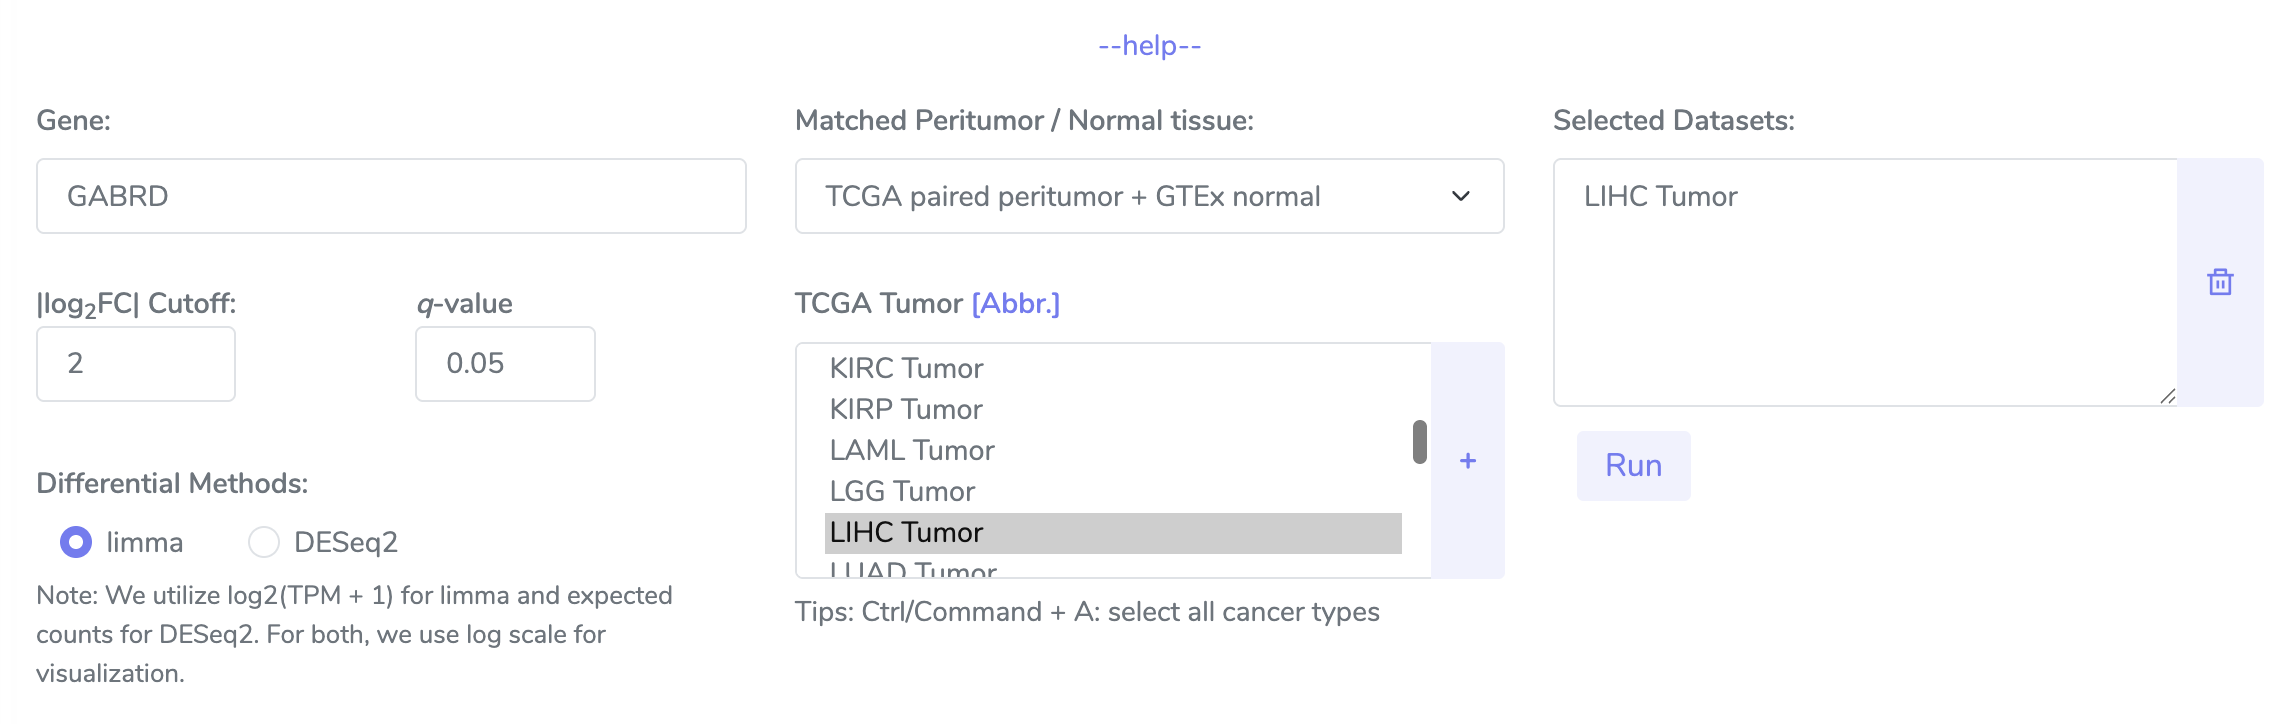
\includegraphics[width=0.5\linewidth]{11.png}
    \caption{GABRD运行界面}
    \label{GABRD运行界面}
\end{figure}

\begin{figure}[H] 
    \centering
    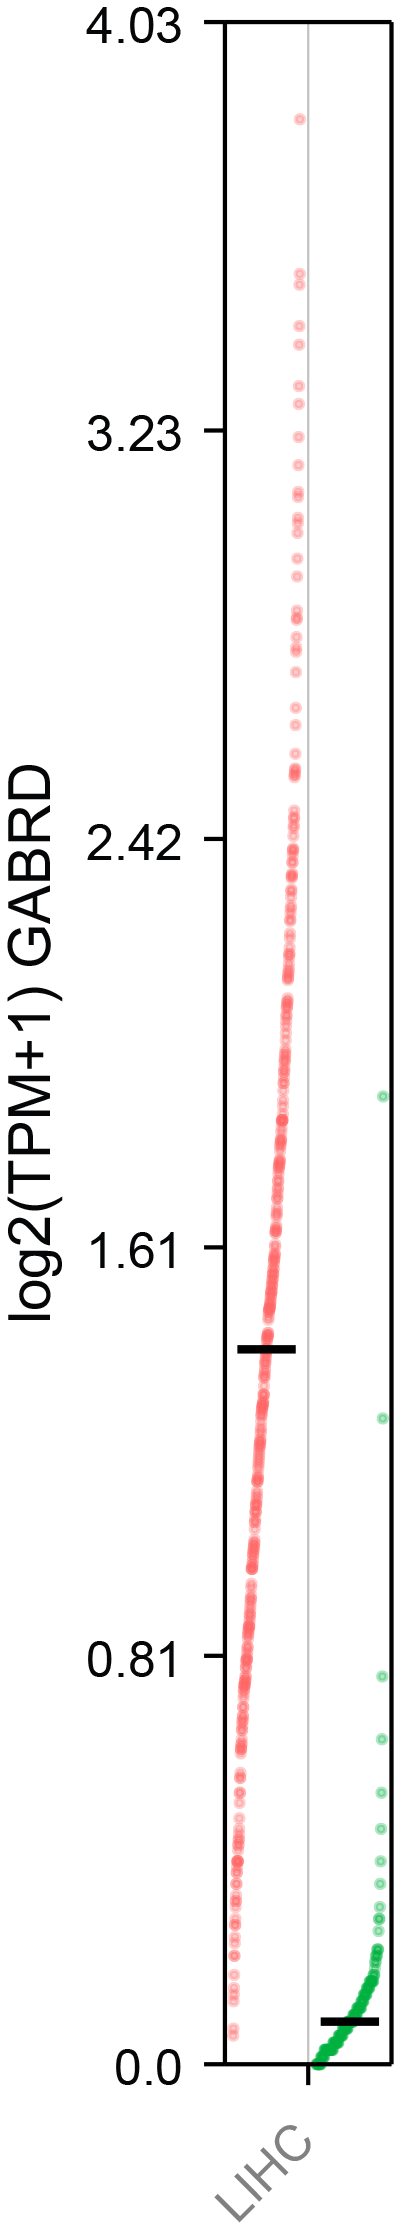
\includegraphics[width=0.1\linewidth]{12.png}
    \caption{GABRD差异表达分析结果分类统计}
    \label{fig:GABRD_de_summary}
\end{figure}

\subsubsection{显著下调基因：ADAMTS13}

在统计结果中，ADAMTS13基因（ENSG00000160323）呈现出了显著下调。利用\href{https://gepia3.bioinfoliu.com/}{gepia3网站}进行外部数据集验证，证明该基因的确在癌症患者体内显著下调。

经过调查发现，ADAMTS13（A Disintegrin And Metalloproteinase with Thrombospondin motifs 13） 是一种分泌型金属蛋白酶编码基因，主要在肝脏产生。ADAMTS13在肝细胞癌中下调，因肝细胞功能丧失及分化降低导致其合成减少；同时肿瘤相关炎症与缺氧抑制其表达。其降低削弱对vWF的裂解，促进微血栓形成与肿瘤血管异常，利于肿瘤生长与转移。

\begin{figure}[H] 
    \centering
    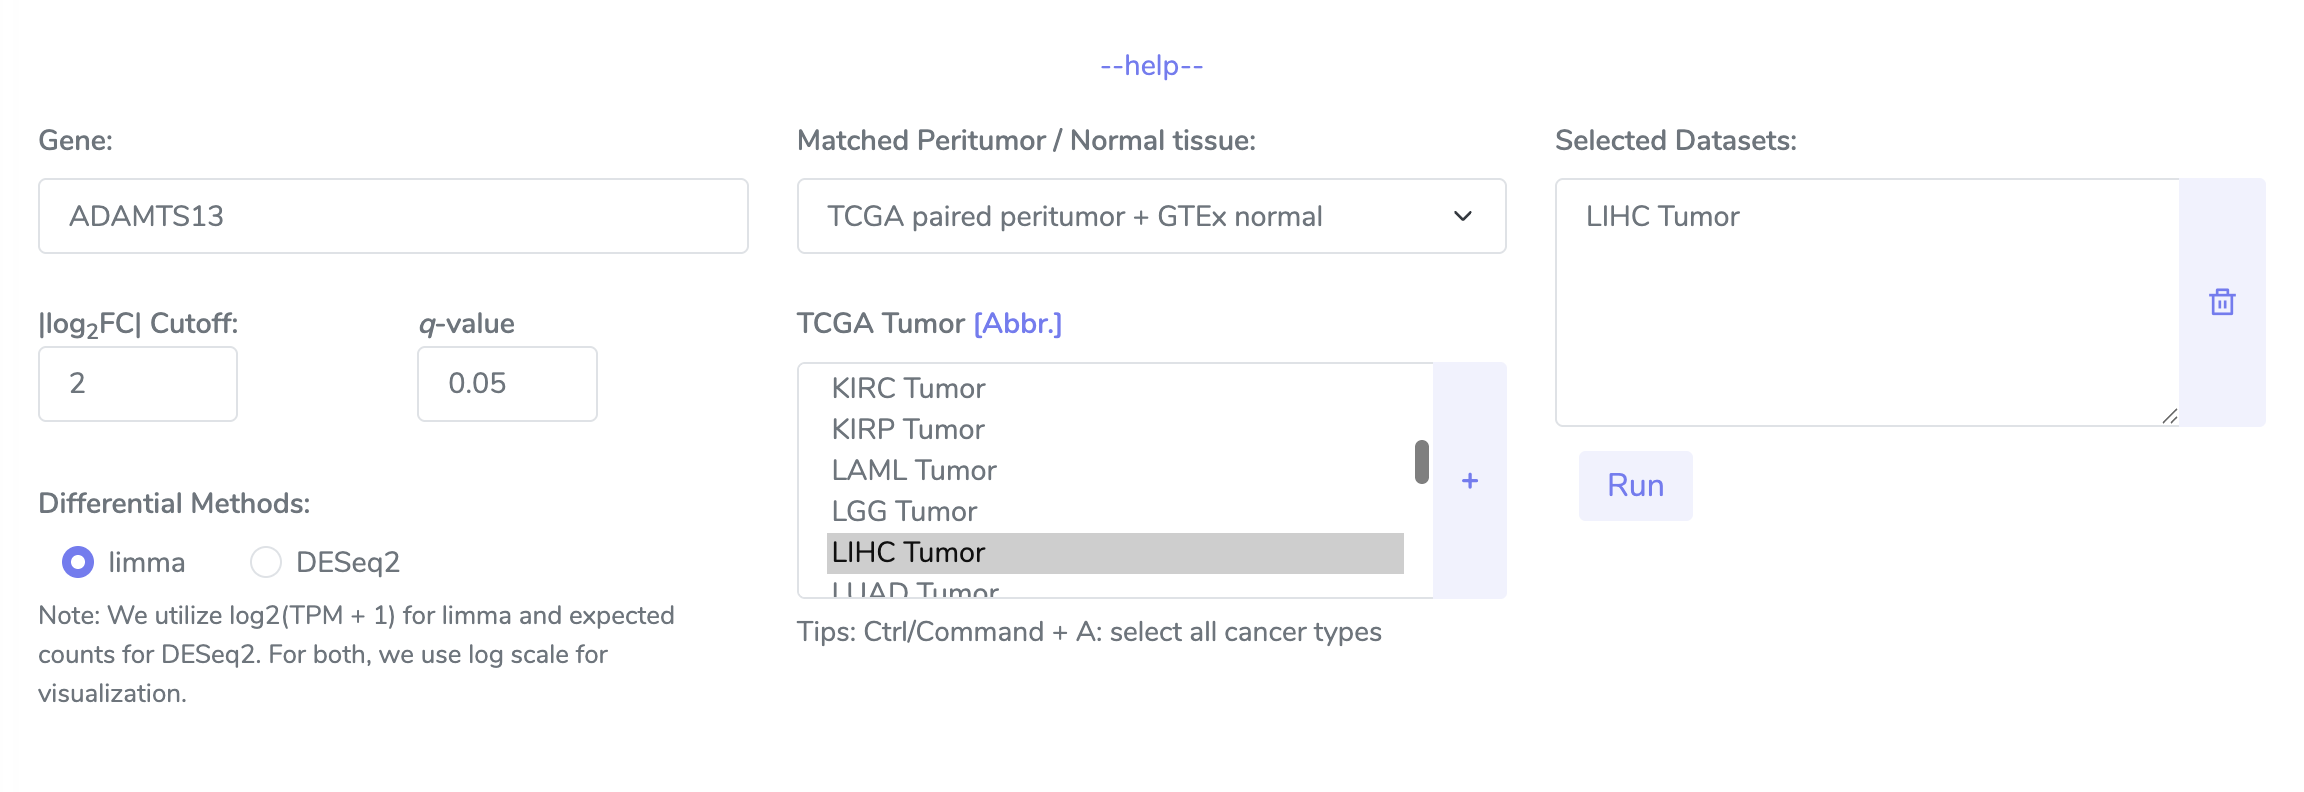
\includegraphics[width=0.5\linewidth]{13.png}
    \caption{ADAMTS13运行界面}
    \label{ADAMTS13运行界面}
\end{figure}

\begin{figure}[H] 
    \centering
    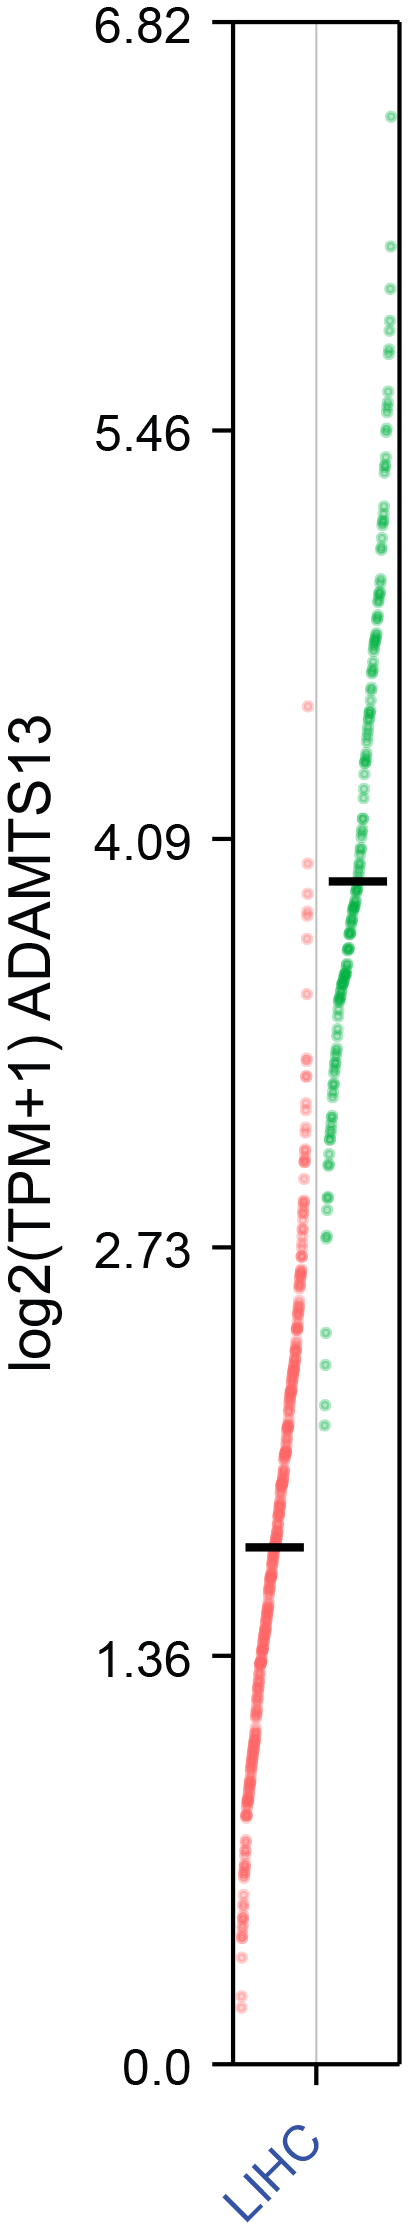
\includegraphics[width=0.1\linewidth]{14.png}
    \caption{ADAMTS13差异表达分析结果分类统计}
    \label{fig:ADAMTS13_de_summary}
\end{figure}

\subsection{拓展调研}

进一步地，将前10个显著上调的基因利用\href{https://gepia3.bioinfoliu.com/survanl/uni/#surv_result}{gepia3网站}进行单变量分析 (Univariable Analysis)。发现基因差异表达的显著性和生存预后并不存在绝对的相关性。在前10个显著上调基因中，最为关键的预后危险因子为KIF2C，其Kaplan-Meier 生存曲线体现了高表达患者有更短的总生存期，这与DEG分析结果相呼应：

\begin{figure}[H] 
    \centering
    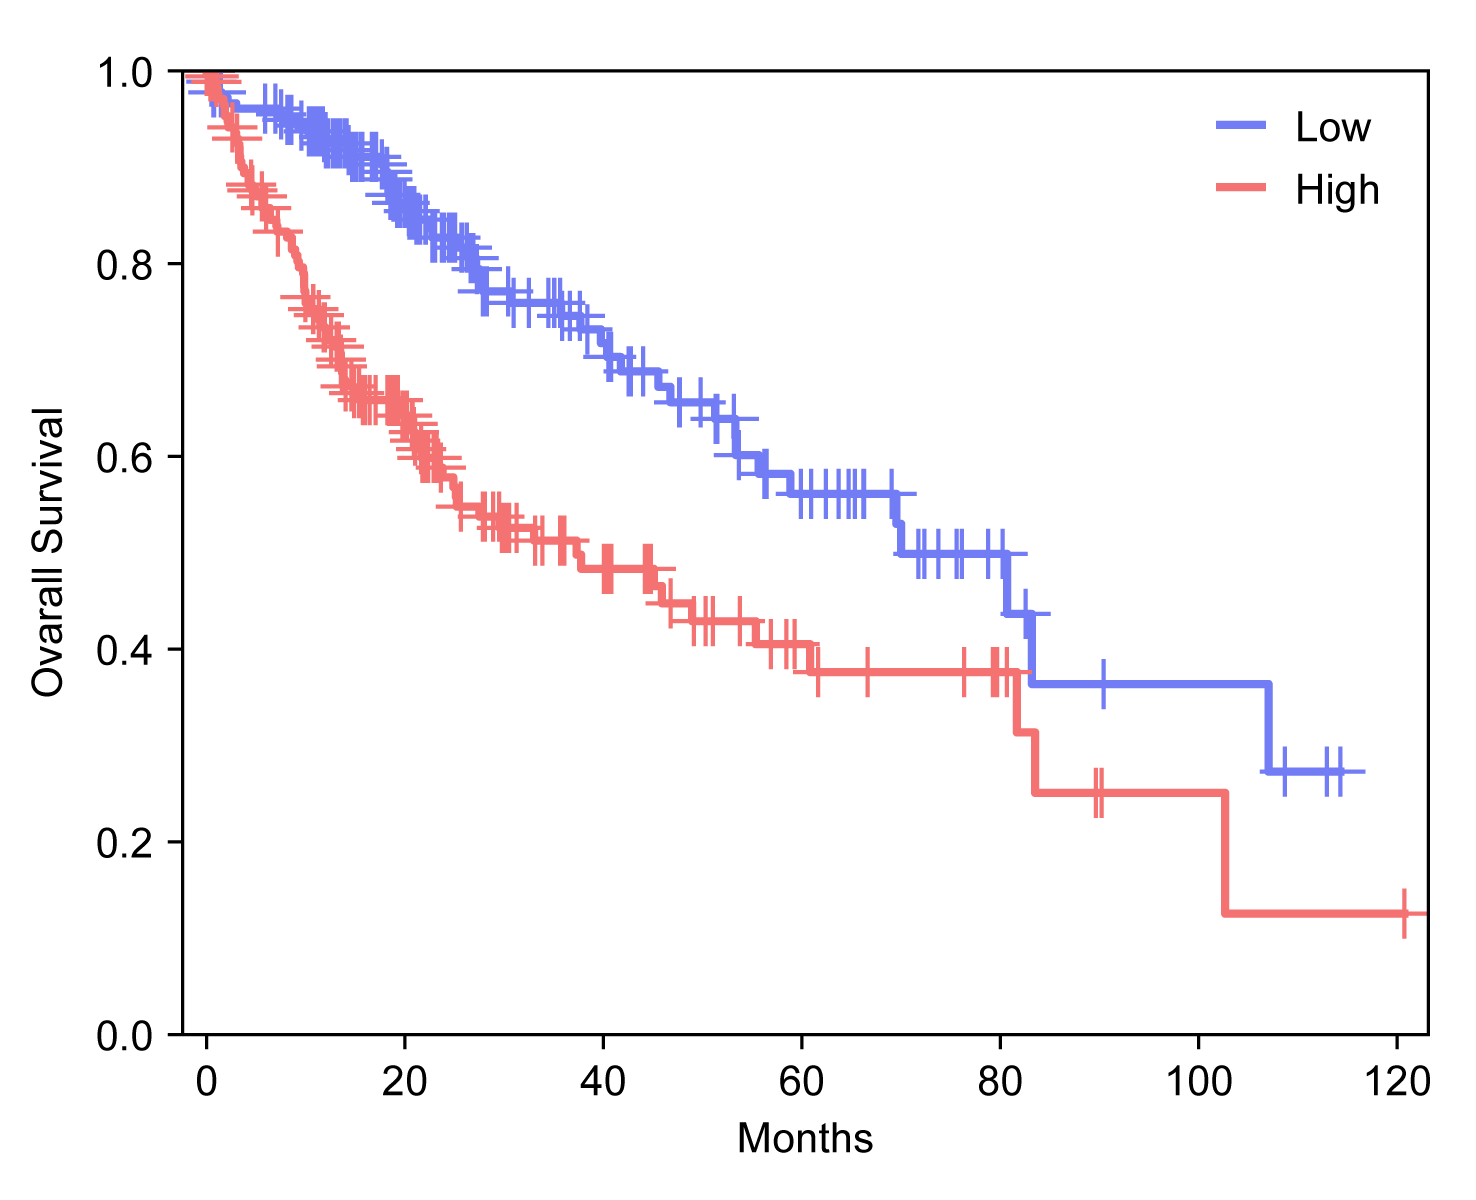
\includegraphics[width=0.5\linewidth]{15.png}
    \caption{KIF2C Kaplan-Meier 生存曲线}
    \label{fig:KIF2C_survival}
\end{figure}

结果显示，该基因风险倍数 (HR)为2.20。表明KIF2C 高表达组的死亡风险是低表达组的 2.20 倍。其低表达组的中位生存期为 70.01 个月，高表达组骤降至 37.29 个月（几乎缩短了一半）。统计显著性 ($P < 0.001$)： $p$ 值和 $p(HR)$ 均远小于 0.05（$1.08 \times 10^{-5}$），说明两组之间的生存差异具有极强的统计学意义，而非随机误差。总结来说，KIF2C 是肝细胞癌（LIHC）的关键预后危险因子，具备高度的临床诊断与监测价值。

KIF2C是驱动蛋白家族的一员，核心功能是调节微管的解聚。在 LIHC 细胞中，KIF2C基因过表达会导致细胞周期的加速，促使癌细胞不受控制地增殖，同时在此过程中会增加染色体错配率，从而加剧肿瘤的异质性和进化能力。

\section{讨论}

\subsection{出现的bug以及解决}

在最开始的代码中，意外出现了结果中存在大量重复基因的问题，在我对DEG结果进行排序后输出的具体结果呈现如下：

\begin{figure}[H] 
    \centering
    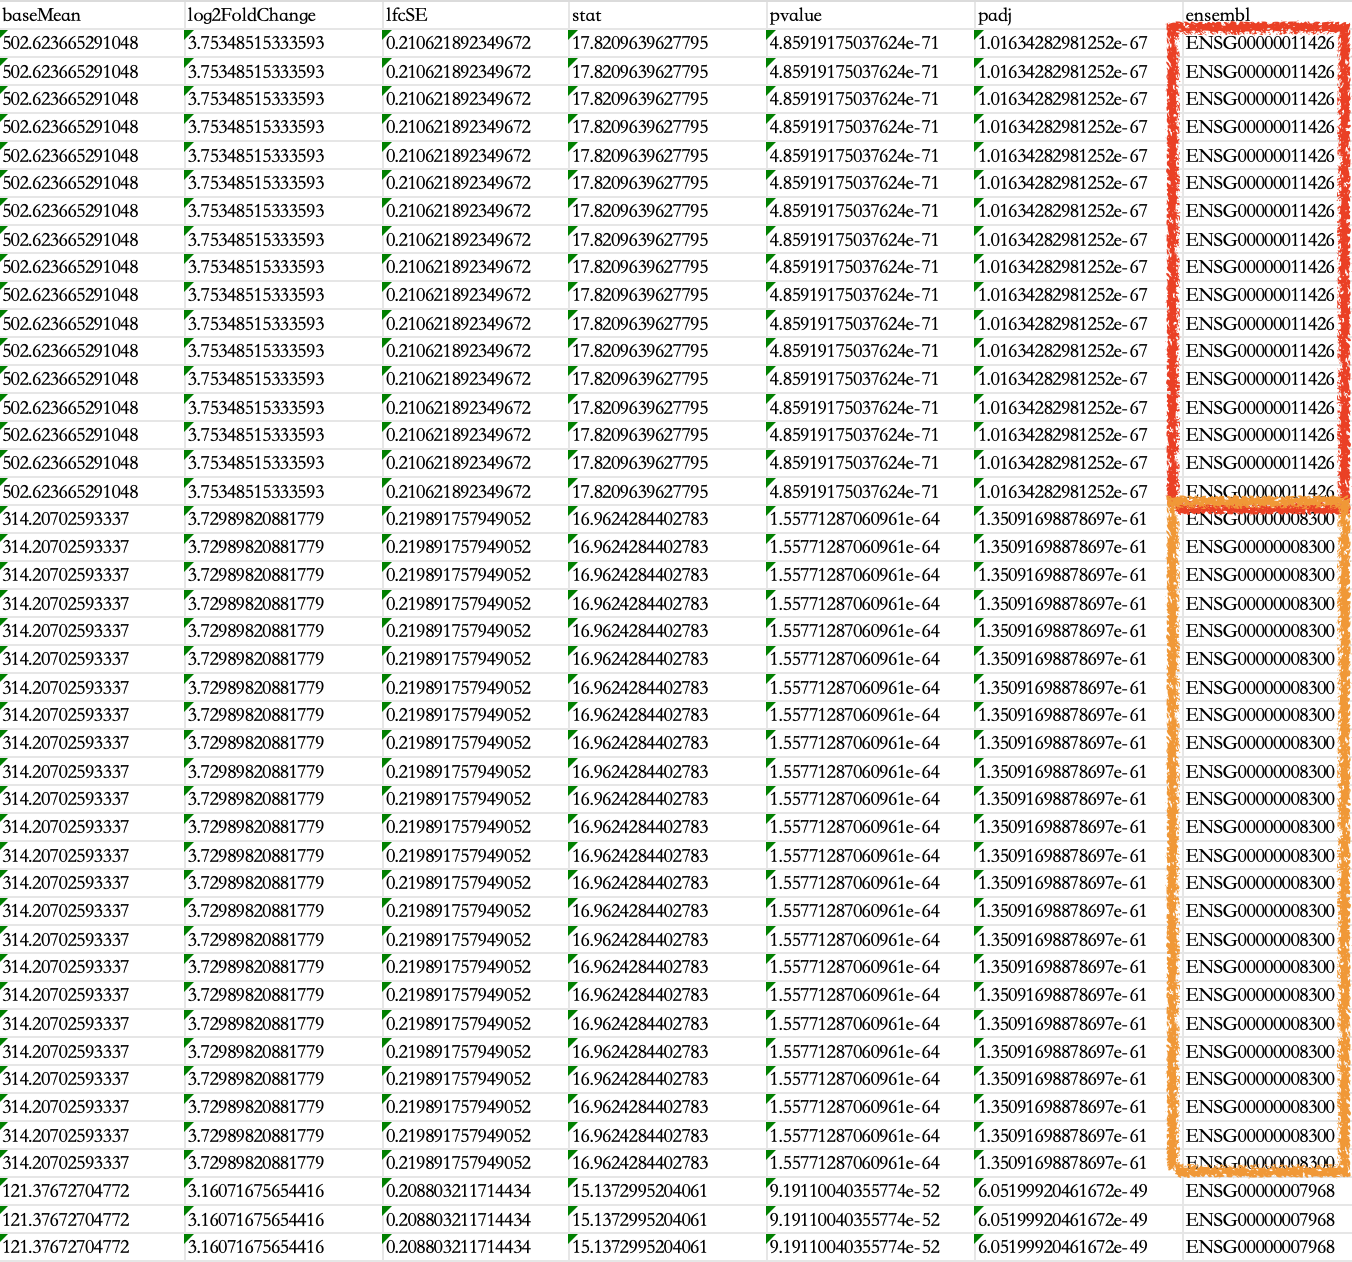
\includegraphics[width=0.5\linewidth]{16.png}
    \caption{错误结果展示}
    \label{fig:wronganswer}
\end{figure}

这说明在代码的某一个步骤出现了错误。在将每一步结果依次输出比对以及重新检查代码后，发现问题为以下步骤：

\begin{lstlisting}[language=R]
keep <- rowSums(counts(dds)>= 10) 
\end{lstlisting}

进一步地，我对于该命令的含义进行了进一步的学习。\texttt{counts(dds)}代表返回一个基因（行）$×$样本（列）的矩阵，矩阵中的值是每个基因在每个样本中的表达量。\texttt{rowSums()}命令是指在对每一行求和，得到一个向量。在代码中代表每个元素是该基因在所有样本中的总计数，因此\texttt{rowSums(counts(dds) >= 10)}符合本身的筛选目的。
而\texttt{rowSums(counts(dds) >= 10)}则是先进行矩阵元素逐个比较，得到一个逻辑矩阵，判断每个基因在每个样本中表达量是否大于等于10，而下一步求和则是在呈现每个基因在多少个样本中表达量大于等于10。

在前者命令中keep是逻辑向量，后续以此为索引时，每个基因只会被保留一次。在后者命令中，keep 是数值向量，在下一步中会把这些数字当作行号索引，因此会重复选中一些基因。

\subsection{limma分析与DEG分析}

在进行外部数据集验证时选择了limma方法呈现结果，在判断基因上调下调以及显著性方面，limma方法与DESeq2方法的结果基本一致，然而在具体的数值上存在差异。

两种方法利用了不同的数据分布的建模方法，DESeq2基于负二项分布模型，而limma基于线性模型。负二项分布通过准确估计离散参数，分辨生物学差异以及随机分布，产生的假阳性较少，而经验贝叶斯模型通过全基因的整体表现，得到一个“背景方差”，相比于前者，在小样本量中表现更为优异。
由于DESeq2软件最为保守，所以算出来的 $p$ 值通常比较大，这一点在进行外部数据集验证的时候也已经发现。

\subsection{基因差异表达与生存预后}

在拓展调研中提到，基因差异表达的显著性和生存预后并不存在绝对的相关性。基因差异表达着重于理解基因对于某一种癌症的功能相关性，然而生存预后分析聚焦于致病性。
因此不难理解，一个基因在肿瘤中显著上调，只能说明它在肿瘤组织中活跃，而不一定是驱动生存差异的核心因子。
在本研究中发现，GABRD基因的显著表达强于KIF2C基因，但是生存预后分析却呈现出了不同的结果。虽然在大量文献中也提及了GABRD对于生存预后的重要意义，但仅从本研究结果出发分析，GABRD 编码 $\mathrm{GABA}_{A}$ 受体 $\delta$ 亚基，主要涉及神经信号调控，在肝癌中可能参与代谢或信号调节，而不是驱动肿瘤恶性行为的核心因子。
但是KIF2C 是微管去聚合酶，直接调控有丝分裂和细胞增殖，高表达会加快肿瘤生长和转移，因此会对生存预后影响更直接。

\subsection{进一步研究方向}

\begin{enumerate}
    \item 多组学整合分析：可以在这个数据集的基础上，结合 RNA-seq、突变、甲基化等修饰的相关数据，分析几个重要基因的表达调控机制。
    \item 单细胞测序数据分析：利用单细胞 RNA-seq数据集（\href{https://www.ncbi.nlm.nih.gov/gds}{GEO 数据库}），分析 DEG 在不同肿瘤细胞亚群或免疫细胞中的特异表达，揭示细胞异质性。
    \item 转录因子预测：结合公开 ChIP-seq 数据验证预测的转录因子结合位点。
\end{enumerate}

\section{补充信息}

\subsection{AI使用说明}

在本次实验中，向AI提供的prompt主要包括以下几个方面：

\begin{enumerate}
    \item latex格式美化类
    \item 火山图绘制：“请给我一些代码建议，我希望能够在火山图上对一些基因进行特定标注”
    \item symbol转换：“请问如何能将基因编码变为基因名称”
    \item 结果分析：“请帮我对比这两种代码在逻辑上是否存在问题”
\end{enumerate}

\subsection{与小组同学讨论}

通过与本组李鉴哲同学进行讨论，对于代码中出现的bug进行了排查，并且对于结果的分析以及后续的拓展调研也有了更深入的理解。

\end{document}
